\documentclass{my_paper}
\usepackage{ctex}
\usepackage[textwidth=444bp,vmargin=2.5cm]{geometry}%设置页边距
\usepackage{array} %主要是增加列样式选项
\usepackage[dvipsnames]{xcolor}%颜色宏包
\usepackage{graphicx}%图片宏包
\usepackage{amsmath}%公式宏包
\usepackage[T1]{fontenc}    
\usepackage{newtxtext, newtxmath}  %两种使用Times New Roman 字体的方法
\usepackage{subfigure}
\usepackage{tabularx, booktabs} %% Load packages that you use
\usepackage{multirow} %跨行处理
\usepackage{rotating}%横向表格
\usepackage{diagbox}%斜线划分表头

\usepackage { gensymb }
% 打°符号\degree
\usepackage{framed}
\usepackage{listings}
% 代码
\usepackage{color} %red, green, blue, yellow, cyan, magenta, black, white
\usepackage[numbered,framed]{matlab-prettifier}%matlab 代码高亮
\usepackage{mdframed}%另一个边框
% matlab代码样式,使用方法为:
% \lstinputlisting[style=Matlab-editor,linewidth=\textwidth]{code.m}
% 或:
% \begin{lstlisting}[style=matlab-prettifier]
%     %code
% \end{lstlisting}
\renewenvironment{framed}[1][\hsize]
  {\MakeFramed{\hsize#1\advance\hsize-\width \FrameRestore}}%
  {\endMakeFramed}
%   修正framed环境,使之可以变长,用法:
%   \begin{framed}[1.2/textwidth]...

\usepackage{hologo}
\usepackage{gbt7714}
\bibliographystyle{gbt7714-numerical}
% 采用国标参考文献引用
\newcommand{\lunwenbiaoti}{\fontsize{15.75pt}{0}\heiti 基于PID自动控制的暖气房屋控温模型}
\newcommand{\zhaiyao}{\fontsize{14pt}{0}\heiti 摘要}
    
\begin{document}

\lstdefinestyle{python_style}{
 columns=fixed,
 numbers=left,                                        % 在左侧显示行号
 numberstyle=\tiny\color{gray},                       % 设定行号格式
 frame=trbl,                                        % 单线背景边框
 breaklines=true,                                     % 设定LaTeX对过长的代码行进行自动换行
 keywordstyle=\color[RGB]{40,40,255},                 % 设定关键字颜色
 numberstyle=\footnotesize\color{darkgray},
 commentstyle=\it\color[RGB]{0,96,96},                % 设置代码注释的格式
 stringstyle=\rmfamily\slshape\color[RGB]{128,0,0},   % 设置字符串格式
 showstringspaces=false,                              % 不显示字符串中的空格
 language=python,                                        % 设置语言
 basicstyle=\linespread{1.0}\fontsize{10bp}{10bp}\selectfont\ttfamily,                      % 字体字号
 %lineskip=10bp,
 %baselinestretch=1,
}
\newpage
\begin{center}
\lunwenbiaoti

\vspace{2ex}
\zhaiyao
\end{center}

摘要

\begin{guanjianci}
 元胞自动机 \quad 边缘检测 \quad 形状匹配
\end{guanjianci}

%----------- 正文 ----------
%----------- 一、问题重述 ----------
\newpage
\section{一、问题重述}

\subsection{问题背景}

为了给予中小企业现金支持,银行针对中小企业的特点,推出一系列不同的信用贷款。对于实力较强信用较好的企业,银行倾向于提供更加优惠的利率。我们需要针对小微企业的开票情况,建立数学模型来给出银行的信贷策略。


\subsection{问题重述}
经过分析整理,我们需要解决以下问题:
\begin{enumerate}
    \item 对附件1给出有信贷记录的123家企业的信贷风险进行量化分¬析,给出该银行在年度信贷总额固定时对这些企业的信贷策略。
    \item 在问题1的基础上,对附件2中没有信贷记录的302家企业的信贷风险进行量化分析,并给出该银行在年度信贷总额为1亿元时对这些企业的信贷策略。
    \item 综合考虑附件2中各企业的信贷风险和可能的突发因素(例如:新冠病毒疫情)对各企业的影响,给出该银行在年度信贷总额为1亿元时的信贷调整策略。
\end{enumerate}

\section{二、问题分析}
\subsection{问题一的分析}

为了解决问题1,需要利用附件中的小微企业发票数据和信誉评级来构建数学模型,以给出银行在年信贷额固定时的信贷策略。因此,我们利用企业发票数据估计营业额,资金缺口和稳定情况,且结合信用评级来给出信贷策略。因此,我们需要构建模型以解决贷款给谁、贷款多少以及利率多少的问题。

\subsection{问题二的分析}


\subsection{问题三的分析}


%----------- 三、模型假设 ----------
\section{三、模型假设}
%使用代码片段:、jiashe%
\begin{enumerate}
    \item 假设企业发票明细完整无误,没有瞒报漏报。
    
    \textbf{原因:}依据企业的发票开具情况,可以直观显示出一个企业的收入支出。因此通过完整的发票记录,可以得到企业的经营特点。


\end{enumerate}

%----------- 四、符号说明 ----------
\section{四、名词解释与符号说明}
%使用三线表格最好~
\subsection{名词解释}
\begin{enumerate}
    % 名词:、mingci
    \item \textbf{dada}
    
    dsadw
    
    \item \textbf{dsadc}
    
    dasdsas

    
\end{enumerate}
\subsection{符号说明}
以下是本文使用的符号以及含义:
\begin{table}[h]%htbp表示的意思是latex会尽量满足排在前面的浮动格式,就是h-t-b-p这个顺序,让排版的效果尽量好。
    \centering
    \begin{tabular}{p{2.0cm}<{\centering}p{9.0cm}<{\centering}p{2.0cm}<{\centering}}
 %指定单元格宽度, 并且水平居中。
    \hline
    符号 & 说明 & 单位 \\ %换行 
    \hline
    $L_0$ & 仓库长度 &  $m$\\
    
    \hline
    \end{tabular}
\end{table}

%----------- 五、模型的建立与求解 ----------
\section{五、模型的建立与求解}

以下将对提出的三个问题进行建模求解。
\subsection{基于熵权法的银行信贷模型}
\subsubsection{企业还款能力评估}
银行放出贷款后是否能够获得收益,取决于贷款是否能够连本带息如数收回。银行信贷盈利的前提是对企业的还款能力进行有效评估,只有向还款能力较好的企业投放信贷,才会有较低的风险,保证收益来源。

为了衡量企业的还款能力,我们提出以下指标:

\begin{enumerate}
    \item 利润率
    
    利润率\cite{1}在经济学中被解释为总所得和总成本的差额同总成本之间的比值。在题目所给的条件中,结合假设条件,我们认为进项发票的票值代表购买产品的成本,而销项发票的票值代表卖出商品的销售额。利用这一指标,可以判断企业的经营情况,根据统计局的相关数据\cite{2}显示,2019年中小企业营业收入利润率为5.6\%,对于高于这一水平的企业,可视为其有较高的利润水平。我们给出利润率$x_1$的计算公式

    \begin{equation}
    x_1 = \frac{\sum\limits_{t\in T\text{销项}}t-\sum\limits_{t\in T\text{进项}}t}{\sum\limits_{t\in T\text{进项}}t}
    \label{x1}
    \end{equation}

    其中$T$代表发票集合,$T\text{进项},T\text{销项}$分别代表进项和销项发票,$t$代表某一发票的数额,下同。
    \item 有效交易占比
    
    在购买商品时,如果出现质量问题,双方无法协商一致时可以选择退货,这是消费者的权益之一。一家店铺的退货数量较多,可以从侧面反映出其存在问题,无论是商品质量,还是服务是否周全,都可在这一指标中体现,所以我们认为开票金额为正的有效发票是有效交易,计算有效交易的占比以判断经营状况的好坏,给出下面的计算公式:
    \begin{equation}
        x_2 = \frac{card(T_{\text{有效},t>0})}{card(T)}
        \label{x2}
    \end{equation}
    其中分子分母中$T$都来自于同一公司的发票记录。

    \item 供应链丰富度
    
    一个企业不能脱离于其他的企业而孤立存在,每个企业都或多或少向其他企业购买产品或者服务,并向其他企业出售。当企业具有丰富的上下游关系时,其抗风险的能力较高,同样反映出企业的组织管理水平较好。供应链丰富度这个指标,我们定义为与企业发生资金往来的企业数目,可以使用单位代号进行标识统计。给出供应链丰富度$x_3$的计算方法:
    \begin{equation}
    x_3 = card(c_{\text{购方}})+card(c_{\text{销方}})
    \label{x3}
    \end{equation}
    其中$c$代表企业的集合。
    \item 信誉等级
    
    信用评级\cite{3}(信誉等级)的目的是显示受评对象信贷违约风险的大小,一般由某些专门信用评估机构进行。对于已经有信贷记录的企业而言,银行已经具有信用评级,可以作为参考,由于使用A、B、C、D四个字母代表不同的信誉评级,为此将其量化为:
    \begin{equation}
    x_4 = \begin{cases}
        1,A\\
        0.75,B\\
        0.5,C\\
        \text{不予放贷},D\\
    \end{cases}
    \label{x4}
    \end{equation}
    其中信用等级为D的不予放贷,仅为了完整性罗列于此。

    \item 平均单价
    
    平均单价反映了企业流水的规模,银行更偏向于向流水规模更高的公司提供信贷。在所给条件下,我们可以使用进销项的平均金额来计算其平均单价。给出计算式:
    \begin{equation}
    x_5 = \frac{\sum\limits_{t\in T\text{销项}}t+\sum\limits_{t\in T\text{进项}}t}{card(T_{\text{进项}})+card(T_{\text{销项}})}
    \label{x5}
    \end{equation}

\end{enumerate}
企业的还款能力需要综合上述的五个因素来看,因此需要为五个指标赋予权重。为此,我们借鉴Chesser模型\cite{4}的思想,提出了求解权重的方法。首先基于五个自变量列出多元线性回归\cite{5}判别法的一般公式: 
\begin{equation}
Y = \alpha + \beta_1x_1 +\beta_2x_2 +\beta_3x_3 +\beta_4x_4 +\beta_5x_5 
\label{Y}
\end{equation}
其中$\alpha$代表常系数,$\beta$代表比例系数,$Y$代表最终输出结果,即企业是否还款。各项$x$的数值已在前文说明,总结如下:
$$\begin{cases}
    x_1 = \frac{\sum\limits_{t\in T\text{销项}}t-\sum\limits_{t\in T\text{进项}}t}{\sum\limits_{t\in T\text{进项}}t}\\
    x_2 = \frac{card(T_{\text{有效},t>0})}{card(T)}
        \\
        x_3 = card(c_{\text{购方}})+card(c_{\text{销方}})
    \\x_4 = \begin{cases}
        1,A\\
        0.75,B\\
        0.5,C\\
        \text{不予放贷},D\\
    \end{cases}\\
    x_5 = \frac{\sum\limits_{t\in T\text{销项}}t+\sum\limits_{t\in T\text{进项}}t}{card(T_{\text{进项}})+card(T_{\text{销项}})}
    \\
\end{cases}$$

我们输出的结果应当是企业是否还贷款,只有“是”和“否”两个选项。是一个典型的二分类问题,认为0为不还贷款,1为还贷。这样待求出的系数可以使用多元线性回归的工具求出。

在得到多元线性回归方程(\ref{Y})后,为了进行预测还贷情况,需要将$Y$映射到$[0,1]$区间内,以符合数理统计的规律。所以在多元线性回归的基础上引入Logit变换,其步骤如下:

\begin{enumerate}
    \item 首先引入比例数(Odds)的概念,企业可以还款的概率为$P$,则其比例数定义为下式:
    \begin{equation}
    Odds = \frac{P}{1-P}
    \label{odd}
    \end{equation}
    \item 对其取对数,得到$\theta$。
    \begin{equation}
        \theta = \ln Odds = \ln \frac{P}{1-P}
        \label{theta}
    \end{equation}
    \item 对式(\ref{theta})变形后,得到概率$P$与$\theta$之间的关系:
    \begin{equation}
        P = \frac{1}{1-\mathit{e}^{-\theta}}
    \end{equation}
\end{enumerate}
Logit 模型事实上就是将线性回归的输出$Y$视作与$\theta$等同,这样最终输出结果在0-1之间,符合要求。因此估计一家企业的获得贷款的概率$P$由下式计算:
\begin{equation}
    \begin{aligned}
        P &= \frac{1}{1-\mathit{e}^{-Y}}\\
        Y &= \alpha + \beta_1x_1 +\beta_2x_2 +\beta_3x_3 +\beta_4x_4 +\beta_5x_5 \\
    \end{aligned}
\label{py}
\end{equation}

综上所述,在针对一名用户判断是否放贷时,首先判断其信用评级是否为$D$若是,则不予放贷,若不是,则利用式(\ref{py})来求解,得到概率$P$若大于0.5则认为可以贷款,若反之,则不予放贷。流程如下图所示:
\begin {figure}[h]
\centering % 居中显示
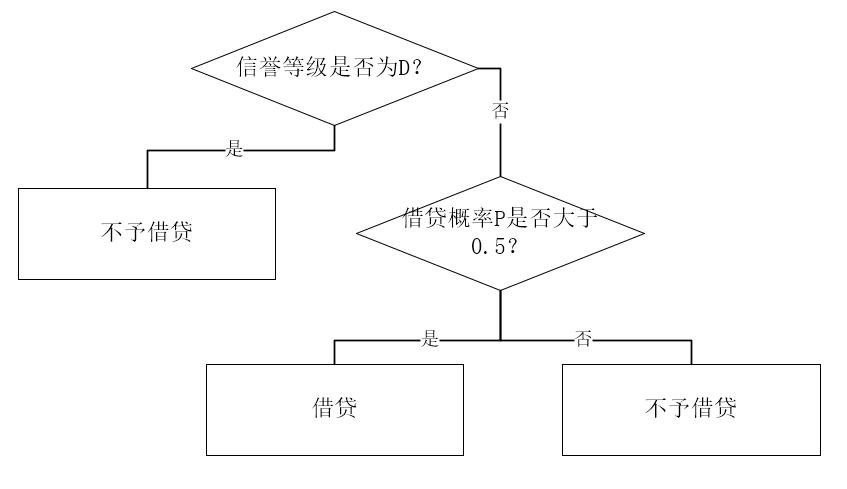
\includegraphics[width=0.8\textwidth]{511.png}
\caption{银行信贷判断图} % 标题
\label{five}
\end {figure}
\newpage
\subsubsection{贷款数量界定}
中小企业由于其经营策略的不同,需要周转的资金数量也有差异。界定中小企业的贷款需求,精准投放有限的资金储备,是银行需要解决的问题。在完成发放贷款与否的界定后,我们将使用熵权法来给出企业贷款数额的界定。

为了更好的判断借款数额,不仅需要利用式(\ref{x1}-\ref{x5})所定义的数值,还需要引入企业的资金缺口$x_6$作为附加的变量。企业在经营的过程中,遵循着先投入后产出的规律,只有首先购进材料产品等,随后售卖盈利,在这一过程中,存在一段时间企业投入资金大于收入所得。在这段时间内产生的支出与获利之差我们定义为资金缺口。当企业获得贷款能够补齐资金缺口时,便可以顺利保证经营的正常进行。我们记录资金缺口为:
\begin{equation}
    x_6 =\sum\limits_{t\in T\text{缺口进项}}t-\sum\limits_{t\in T\text{缺口销项}}t
\label{x6}
\end{equation}

对于许多小企业而言,需要使用同一套标准来计算其贷款额度。计算的依据是$x_1,/cdots,x_6$这六个指标,分别代表利润率,有效交易占比,供应链丰富度,信誉等级,平均单价,资金缺口六个要素。这六个要素量纲不同,数值不同,需要利用熵权法来给定各个因素在贷款分配策略中所占有的权重。其具体步骤如下:

\section{六、敏感性分}
\section{七、模型的评价}

\subsection{模型的优点}
\begin{enumerate}
    \item 采用

\end{enumerate}

\subsection{模型的缺点}
\begin{itemize}
    \item 利用较

\end{itemize}

%----------- 参考文献 ----------
\newpage
\begin{center}
\bibliography{reference} %调出LaTeX生成参考文献列表
\end{center}

%----------- 附录 ----------
\newpage
\section{附件}
\textbf{附件清单:}
\renewcommand\theenumi{\roman{enumi}}
% 规定数字格式为罗马数字
\renewcommand\labelenumi{\textbf{附录\theenumi}}
% 规定是附录某某
\begin{itemize}
    \item xxx代码
\end{itemize}

\textbf{sobel边缘检测代码}

\begin{lstlisting}[language=matlab]
    function GAdsa 
\end{lstlisting}



\end{document}